\subsection{Cube}

\subsubsection{Facial \& Body diagonal}

Facial diagonal join two vertices at the same face.

Body diagonal join two vertices from opposite faces.

\begin{figure}[H]
  \centering
  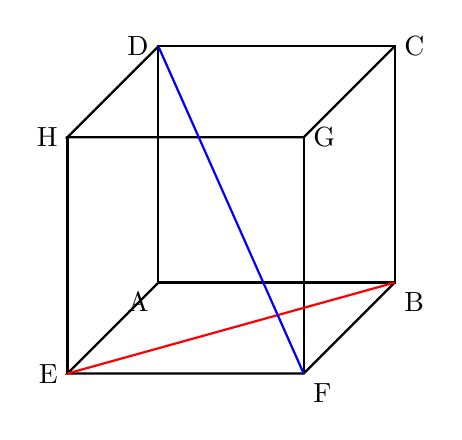
\begin{tikzpicture}[scale=1.5] % Define vertices
    \coordinate (A) at (0,0,0); \coordinate (B) at (2,0,0); \coordinate (C) at (2,2,0); \coordinate (D) at (0,2,0); \coordinate (E) at (0,0,2); \coordinate (F) at (2,0,2); \coordinate (G) at (2,2,2); \coordinate (H) at (0,2,2);

    % Draw edges
    \draw[thick] (A)--(B)--(C)--(D)--cycle;
    \draw[thick] (A)--(E)--(F)--(B);
    \draw[thick] (C)--(G)--(H)--(D);
    \draw[thick] (E)--(H)--(G)--(F);

    % Add vertex labels
    \node[below left] at (A) {A};
    \node[below right] at (B) {B};
    \node[right] at (C) {C};
    \node[left] at (D) {D};
    \node[left] at (E) {E};
    \node[below right] at (F) {F};
    \node[right] at (G) {G};
    \node[left] at (H) {H};

    % Draw facial diagonal
    \draw[thick,red] (E)--(B);

    % Draw body diagonal
    \draw[thick,blue] (F)--(D);

  \end{tikzpicture}
\end{figure}

\[
  \begin{array}{l}
    \text{Facial diagonal} = L \sqrt{2} \\
    \text{Body diagonal} = L \sqrt{3} \\
  \end{array}
\]

\subsubsection{Area}

\[
  A=6L^2 
\]

\subsubsection{Volume}

\[
  V=L^3 
\]

\subsubsection{Circumscribed sphere}

Pass through the $8$ vertices, radius equal to $L(\frac{\sqrt{3}}{2})$.


%\begin{figure}[H]
%  \centering
%  \begin{tikzpicture}[scale=1.5, line join=round] 
%    \pgfmathsetmacro{\l}{1} % Lado do cubo
%
%    \draw[fill=gray!20] (0,0,0) -- (\l,0,0) -- (\l,\l,0) -- (0,\l,0) -- cycle;
%    \draw[fill=gray!20] (\l,0,0) -- (\l,0,\l) -- (\l,\l,\l) -- (\l,\l,0) -- cycle;
%    \draw[fill=gray!20] (0,0,0) -- (0,0,\l) -- (0,\l,\l) -- (0,\l,0) -- cycle;
%
%    \draw[fill=gray!20] (\l,\l,0) -- (\l,\l,\l) -- (0,\l,\l) -- (0,\l,0) -- cycle;
%    \draw[fill=gray!20] (0,0,\l) -- (\l,0,\l) -- (\l,\l,\l) -- (0,\l,\l) -- cycle;
%
%    \shade[ball color=blue!50!white, opacity=0.5] (0.5*\l,0.5*\l,0.5*\l) circle ({\l*sqrt(3)/2});
%  \end{tikzpicture}
%\end{figure}

\subsubsection{Inscribed Sphere}

Tangent to the $6$ faces, radius equal to $\frac{L}{2}$.

%\begin{figure}[H]
%  \centering
%  \begin{tikzpicture}[scale=1.5, line join=round] 
%    \pgfmathsetmacro{\l}{1} % Lado do cubo
%
%    % Desenhando o cubo
%    \draw[fill=gray!20] (0,0,0) -- (\l,0,0) -- (\l,\l,0) -- (0,\l,0) -- cycle;
%    \draw[fill=gray!20] (\l,0,0) -- (\l,0,\l) -- (\l,\l,\l) -- (\l,\l,0) -- cycle;
%    \draw[fill=gray!20] (0,0,0) -- (0,0,\l) -- (0,\l,\l) -- (0,\l,0) -- cycle;
%
%    \draw[fill=gray!20] (\l,\l,0) -- (\l,\l,\l) -- (0,\l,\l) -- (0,\l,0) -- cycle;
%    \draw[fill=gray!20] (0,0,\l) -- (\l,0,\l) -- (\l,\l,\l) -- (0,\l,\l) -- cycle;
%
%    % Esfera inscrita
%    \shade[ball color=green!50!white, opacity=0.5] (0.5*\l,0.5*\l,0.5*\l) circle ({\l/2});
%
%  \end{tikzpicture}
%\end{figure}

\subsubsection{Tangent Sphere}

Tangent to the edges, radius equal to $\frac{L}{\sqrt{2}}$.

%\begin{figure}[H]
%  \centering
%  \begin{tikzpicture}[scale=1.5, line join=round] 
%    \pgfmathsetmacro{\l}{1} % Lado do cubo
%    \draw[fill=gray!20] (0,0,0) -- (\l,0,0) -- (\l,\l,0) -- (0,\l,0) -- cycle;
%    \draw[fill=gray!20] (\l,0,0) -- (\l,0,\l) -- (\l,\l,\l) -- (\l,\l,0) -- cycle;
%    \draw[fill=gray!20] (0,0,0) -- (0,0,\l) -- (0,\l,\l) -- (0,\l,0) -- cycle;
%
%    \draw[fill=gray!20] (\l,\l,0) -- (\l,\l,\l) -- (0,\l,\l) -- (0,\l,0) -- cycle;
%    \draw[fill=gray!20] (0,0,\l) -- (\l,0,\l) -- (\l,\l,\l) -- (0,\l,\l) -- cycle;
%
%    \shade[ball color=red!50!white, opacity=0.5] (0.5*\l,0.5*\l,0.5*\l) circle ({\l*sqrt(2)/2});
%  \end{tikzpicture}
%\end{figure}
